\chapter{Decision tree learning}
From data is sometime possible to build a tree of features that allows to find an item's target value: given an example, with respect to the values the example assumes for each feature, it's possible to build a path which will lead to a leaf, that is a label.
\begin{center}
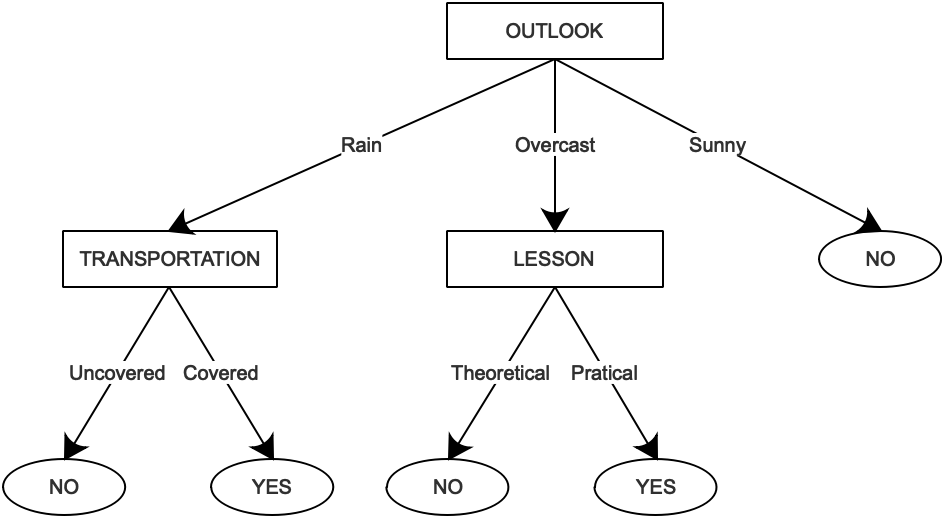
\includegraphics[width=0.9\linewidth]{DecisionTree}
\end{center}
A tree is a disjunction of conjunctions of constraints over attribute values, that is it express a disjunction normal form. Each path from the root to a leaf is a conjunction of hte constraints specified in the nodes along it, e.g., if it's cloudy and the lesson is theoretical, then a student is not going to go to the lesson.
\begin{center}
	$\displaystyle \text{OUTLOOK}=\text{Overcast}\wedge \text{LESSON}=\text{Theoretical}$
\end{center}
One of the strongest advantages of this model is its explainability: it's easy to know what the model does and what the outcome may be. \newline
Such representation works best with binary and multiclass classification takes, even though some extensions to regression also exists, for example exploiting means properties. Another field in which it works fine is with missing attribute, that is for example when some feature don't have any value. \newline
%
%
%
\section{Algorithm}
The learning algorithm in this case is simply a greedy approach proposes by Quinlan: for each node, starting from the root:
\begin{enumerate}
	\item Choose the best attribute to be evaluated;
	\item Add a child for each attribute value;
	\item Split node training set into children according to value of chosen attribute;
	\item Stop splitting a node if it contains examples from a single class, or there are no more attribute to test.
\end{enumerate}
The idea is to start with a whole training set and then choose the feature so that the set will become as parted as possible. We stop when the example in the training set are all of the same class or there are no more features to be tested.\newline 
%
%
\subsection{Choosing the best attribute}
The best strategy to choose the best attribute on which to split, is to use sets' \textbf{homogeneity}, which is based on the concept of \textbf{entropy}.
\begin{definition}[Entropy]
Entropy is a measure of the amount of information contained in a collection of instances $S$ which can take a number $c$ of possible values:
\begin{center}
	$\displaystyle H(S)=-\Sum_{i=1}^cp_i\log_2(p_i)$
\end{center}
Where $p_i$ is the fraction of $S$ taking value $i$. 
\end{definition}
Entropy is the way in which the increment of homogeneity is measured since it's based on the information contained in a set: if all the values inside the set are the same, then there is no information, otherwise if two values are one the opposite of the other, then there is maximum entropy since the probability of taking one or the other becomes $5\%$.\newline
Given the entropy then it's possible to compute the \textbf{information} fain:
\begin{definition}[Information Gain]
The information gain $IG$ is the expected reduction in entropy obtained by partitioning a set $S$ according to the value of a certain attribute $A$:
\begin{center}
	$\displaystyle IG(S, A)=H(S)-\Sum_{v\in Values(A)}\frac{\abs{S_v}}{\abs{S}}H(S_v)$
\end{center}
\end{definition}
The greater the difference (IG), the better it is.
%
%
\subsection{Overfitting}
With decision tree it's possible to end up with overfitting for example when from each set of $n$ elements, only one element is selected at the time. In this way the leaves would just contain one example creating a complex tree and leading to overfitting. \newline
So the goal is not to obtain pure leaves, but instead to have also leaves that can contains example not strictly from that class.\newline
There are two ways to avoid this possibility in decision trees:
\begin{itemize}
	\item \textbf{Pre-pruning}: decide whether to stop splitting a node even if it contains training example with different labels.
	\item \textbf{Post-pruning}: learn a full tree, risking overfitting, and then in case prune to remove subtrees. Usually this strategy is the one used.
\end{itemize}
Let's focus on the post-pruning strategy: for this we shall introduce a validation set, that is a set against which to test the trained model. Let's consider a full tree, then:
\begin{enumerate}
	\item For each node in the tree: evaluate the performance on the validation set when removing the subtree rooted at it;
	\item If all node removals worsen performance, then stop;
	\item Choose the node whose removal has the best performance improvement;
	\item Replace the subtree rooted at it with a leaf;
	\item Assign to the leaf the majority label of all examples in the subtree;
	\item Return to 1.
\end{enumerate}
When no more improvements are obtained through pruning, then the pruning is finished. \newline
Obviously validation, training and test set must all have the same statistics.\newline
%
%
%
\section{Problem with decision tree}
%
%
\subsection{Discretization}
A first problem with decision trees are continuous-valued attributes. One easy solution is to discretize the variable in order to be used in the internal nodes tests. \newline
Discretization implies the usage of thresholds, which can be set in order to maximize the attribute quality criterion, e.g. information gain. \newline
The procedure to achieve this is:
\begin{itemize}
	\item Examples are sorted according to their continuous attribute values;
	\item For each pair of successive examples having different labels, a \textit{candidate threshold} is places ad the average of the two attribute values.
	\item For each candidate threshold, the information gain is achieved splitting examples according to how it is computed;
	\item The threshold producing the higher information gain is used to discretize the attribute. 
\end{itemize}
%
\subsubsection{Example}
Let's suppose that we want to accept a work based on the age via the following table:
\begin{center}
\begin{tabular}{c|c}
	age&class\\
	23&y\\
	27&y\\
	34&n\\
	38&n\\
	35&y\\
	32&n\\
\end{tabular}
\end{center}
As a first thing, ordering data can be a great deal:
\begin{center}
\begin{tabular}{c|c}
	age&class\\
	23&y\\
	27&y\\
	32&n\\
	34&n\\
	35&y\\
	38&n\\
\end{tabular}
\end{center}
Then a threshold can be chosen, for example in the point where the class changes, even if some other examples are present afterwards, so for example age=32 can be a threshold.\newline
%
%
\subsection{Alternative attributes test measures}
Information gain has a problem: if for example the set contained people with an id, it would place each person into a leaf, because this would make the information gain as big as possible. \newline
Information gain works fine, but in some cases it divides too much. \newline

In order to avoid the tree from becoming too much spread, it's possible to measure the entropy with respect to the attribute value instead of the class value:
\begin{center}
	$\displaystyle H_A(S)=-\Sum_{v\in Values(A)}\frac{\abs{S_v}}{\abs{S}}\log_2\frac{\abs{S_v}}{\abs{S}}$
\end{center}
Bigger the entropy, bigger is the division the attribute is making of the tree.\newline
Now instead of using the information gain, we could downweight it with respect to the new entropy and compute the \textbf{gain ratio}:
\begin{center}
	$\displaystyle IGR(S,A)=\frac{IG(S,A)}{H_A(S)}$
\end{center}
%
%
\subsection{Missing values}
At the beginning we said that decision trees could deal also with missing values. Let's suppose that at a certain node $n$ we'd like to split on attribute $A$, but the example $x$ of class $c(x)$ is missing its value for attribute $A$. Two solutions are possible:
\begin{itemize}
	\item Simple: assign to $x$ the most common attribute values among examples in $n$, or the most common of examples in $n$ with class $c(x)$. This works in every condition, but it's not very performing.
	\item Complex: propagate $x$ to each of the children of $n$ with a fractional value equal to the proportion of example with the corresponding attribute value. This implies that at test time, for each candidate class, all fractions of the test example which reached a leaf with that class are summed, and the example is assigned the class with the highest overall value. 
\end{itemize}
%
%
%
\section{Random Forests}
The decision trees are easy to be used, but not really great in terms of accuracy. An extension of the decision trees is random forests. \newline
Given a set of $N$ examples, sample $N$ examples with replacement, that is the same example can be selected multiple times. Then train a decision tree on the sample, selecting at each node $m$ features at random among which to choose the best one. Repeat this procedure multiple times to generate a forest with multiple trees.\newline
As for the testing, each example is tested against each tree in the forest, and the majority class among the predictions is returned. 